\documentclass[10pt]{article}
\usepackage[polish]{babel}
\usepackage[utf8]{inputenc}
\usepackage[T1]{fontenc}
\usepackage{amsmath}
\usepackage{amsfonts}
\usepackage{amssymb}
\usepackage[version=4]{mhchem}
\usepackage{stmaryrd}
\usepackage{graphicx}
\usepackage[export]{adjustbox}
\graphicspath{ {./images/} }

\title{GIMNAZJUM }

\author{}
\date{}


\begin{document}
\maketitle
\begin{enumerate}
  \item Punkty \(K\) i \(L\) leżą na bokach \(A D\) i \(B C\) równoległoboku \(A B C D\), przy czym \(A K=L C\). Punkt \(P\) leży na boku \(C D\). Pokazać, że jeśli prosta \(K L\) przecina proste \(A P\) i \(B P\) odpowiednio w punktach \(M\) i \(N\), to pole trójkąta \(P M N\) jest równe sumie pól trójkątów \(A K M\) i BLN.\\
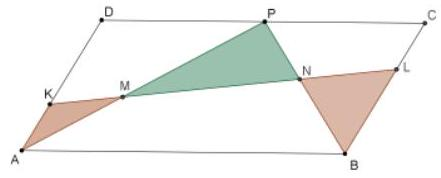
\includegraphics[max width=\textwidth, center]{2024_11_21_c99ffd375c316295e466g-1}
  \item Budowane pomieszczenie w kształcie prostopadłościanu ma mieć wysokość 3 m , podłoga zaś ma mieć wymiary \(3 \mathrm{~m} \times 7,5 \mathrm{~m}\). W pomieszczeniu nie będzie okien, jedynie drzwi na jednej kwadratowej ścianie. Prąd do pomieszczenia ma być doprowadzony nad drzwiami, 25 cm pod sufitem, w odległości \(1,5 \mathrm{~m}\) od obu sąsiednich ścian. Jedyne gniazdko ma natomiast być umieszczone na przeciwległej ścianie, też w odległości \(1,5 \mathrm{~m}\) od obu sąsiednich ścian, ale 25 cm nad podłogą. Jak, chcąc zużyć jak najmniej kabla, poprowadzić go od puszki z prądem do kontaktu? Oczywiście kładziemy kabel przed otynkowaniem i położeniem podłogi, a poprowadzenie go bezpośrednio od puszki do gniazdka, po linii prostej przez środek pokoju, jest wykluczone.
  \item W turnieju tenisa stołowego wzięło udział 50 zawodników. Każdy zawodnik rozegrał jeden mecz z każdym innym zawodnikiem, nie było remisów. Czy możliwe jest, aby każdy z uczestników wygrał tę samą liczbę meczów? Odpowiedź uzasadnij.
\end{enumerate}

\section*{LICEUM}
\begin{enumerate}
  \item Na każdym polu szachownicy \(2012 \times 2012\) mieszka krasnoludek, przy czym żaden z krasnoludków nigdy nie opuszcza pola, na którym mieszka. Okazało się, że 2016 krasnoludków cierpi na nieuleczalną, zaraźliwą chorobę - matemafilię, w tym 16 krasnoludków mieszkających na kwadracie \(4 \times 4\) na samym środku szachownicy. Zdrowy krasnoludek zarazi się matemafilią, jeśli co najmniej dwóch jego sąsiadów jest na nią chorych (sąsiadami są krasnoludki, które zajmują pola o sąsiednim boku). Zarażenie matemafilią następuje zawsze o północy, przy czym zarażony krasnoludek może zarazić innego dopiero po 12 godzinach. Czy jest możliwe, że wszystkie krasnoludki będą chore na matemafilię? Jeśli tak, to po ilu - najpóźniej - dniach się to stanie?
  \item Znajdź wszystkie trójki liczb całkowitych nieujemnych \(a, b, c\) spełniające układ równań:
\end{enumerate}

\[
\left\{\begin{array}{l}
a+b c=3 b \\
b+c a=3 c \\
c+a b=3 a
\end{array}\right.
\]

\begin{enumerate}
  \setcounter{enumi}{2}
  \item Punkt \(M\) jest środkiem przeciwprostokątnej \(A B\) trójkąta prostokątnego \(A B C\). Symetralna odcinka \(C M\) przecina proste \(A C\) i \(B C\) odpowiednio w punktach \(K\) i \(L\). Wykaż, że \(A K^{2}+B L^{2}=K L^{2}\)\\
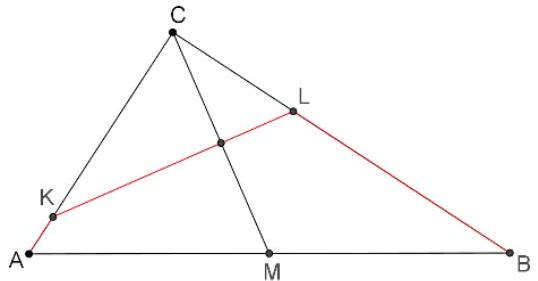
\includegraphics[max width=\textwidth, center]{2024_11_21_c99ffd375c316295e466g-1(1)}
\end{enumerate}

Rozwiq̨zania należy oddać do piqtku 10 kwietnia do godziny 12.30 koordynatorowi konkursu panu Jarosławowi Szczepaniakowi lub swojemu nauczycielowi matematyki.


\end{document}